
%(BEGIN_QUESTION)
% Copyright 2006, Tony R. Kuphaldt, released under the Creative Commons Attribution License (v 1.0)
% This means you may do almost anything with this work of mine, so long as you give me proper credit

An RTD measures the temperature of saturated steam at the steam drum of a boiler:

$$\includegraphics[width=15.5cm]{i00653x01.eps}$$

The RTD connects to a bridge circuit via three wires, to register temperature at a sensitive voltmeter mechanism in the control room:

$$\includegraphics[width=15.5cm]{i00653x02.eps}$$

Suppose the boiler operator decides to decrease the pressure of the boiler over a period of time.  Identify the effects this pressure change will have on these voltage drops in the RTD circuit:

\begin{itemize}
\item{} $V_{R1}$ will {\it increase}, {\it decrease}, or {\it stay the same}?
\item{} $V_{R2}$ will {\it increase}, {\it decrease}, or {\it stay the same}?
\item{} $V_{R3}$ will {\it increase}, {\it decrease}, or {\it stay the same}?
\item{} $V_{RTD}$ will {\it increase}, {\it decrease}, or {\it stay the same}?
\item{} Explain the relationship between boiler pressure and boiler temperature:
\end{itemize}

\underbar{file i00653}
%(END_QUESTION)





%(BEGIN_ANSWER)

\begin{itemize}
\item{} $V_{R1}$ will {\bf stay the same}
\item{} $V_{R2}$ will {\bf stay the same}
\item{} $V_{R3}$ will {\bf increase}
\item{} $V_{RTD}$ will {\bf decrease}
\item{} Explain the relationship between boiler pressure and boiler temperature:

\vskip 10pt

{\it Boiler pressure and boiler temperature are directly related: as pressure decreases, temperature also decreases.}

%(END_ANSWER)





%(BEGIN_NOTES)


%INDEX% Measurement, temperature: RTD
%INDEX% Physics, heat and temperature: saturated steam pressure versus temperature

%(END_NOTES)


